\chapter{Wstęp}

\section{Wprowadzenie}
Ochrona Ziemi przed zgubnymi skutkami zanieczyszczeń, właściwa gospodarka odpadami, racjonalne zużycie wody -- to wyzwania, którym ludzka cywilizacja musi czym prędzej stawić czoło. Od wielu już lat podkreślają to różne organizacje oraz społeczności. Za tymi wyzwaniami ukryte są jednak liczne problemy, które spowalniają czy też utrudniają podejmowanie pro-ekologicznych działań. Dotyczą one technologii, kultury, polityki i innych obszarów. Wśród nich szczególne miejsce zajmują problemy motoryzacji. Od dawna podkreśla się negatywny wpływ emisji gazów cieplarnianych oraz wyników spalania paliw na ekologię Ziemi. Zahamowanie trwającej od kilku dziesięcioleci tendencji powinno nastąpić w wyniku zastosowania w samochodach napędów hybrydowych lub czysto elektrycznych. Według różnych źródeł liczba samochodów elektrycznych rośnie z każdym rokiem i ten wzrost powinien utrzymać się przez długi czas (rys. \ref{fig:car_chart}) \cite{iea1,mam1}. Wraz z nimi rośnie potrzeba rozbudowy infrastruktury pozwalającej na szybkie uzupełnianie w tych samochodach energii. 
% TO DO: można byłoby wstawić tu przerysowany wykres, wtedy Cel i zakres pracy wylądowałyby na nowej stronie
% TO VERIFY:
\begin{figure}[ht]
    \centering
        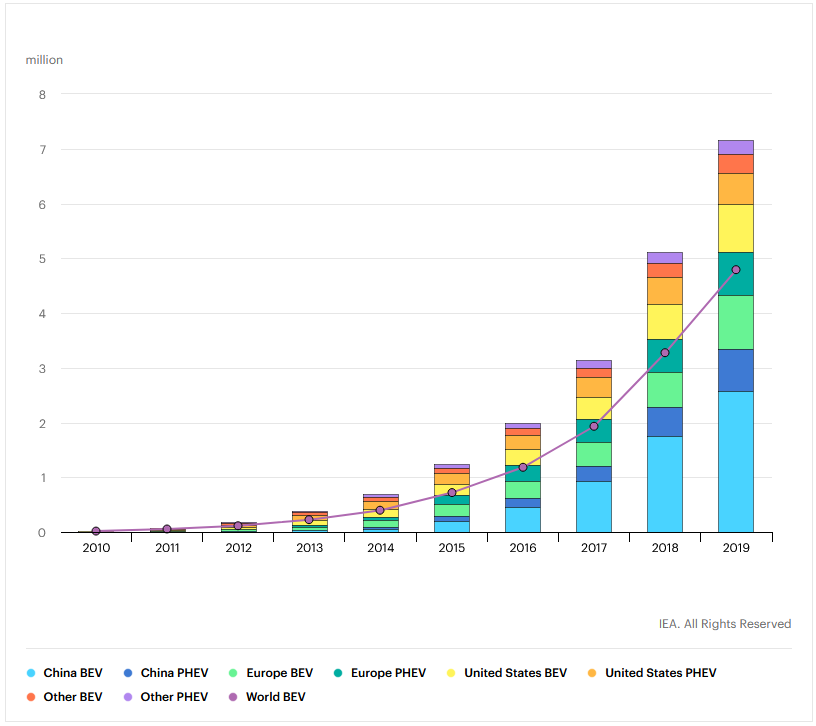
\includegraphics[width=1\linewidth]{rys01/chart.png}
        \caption{Ilość samochodów elektrycznych w różnych krajach z ciągiem czasu \cite{car_chart}}
    \label{fig:car_chart}
\end{figure}

W krajach WNP (Wspólnoty Niepodległych Państw), i być może nie tylko w nich, sporym problemem okazuje się znalezienie stacji do ładowania samochodów elektrycznych. Zdarzają się sytuacje, w których po przybyciu do stacji ładowania stacja ta okazuje się nieczynna lub położona w niedostępnym miejscu (na przykład na prywatnym terenie), a przewody umożliwiające podłączenie się są za krótkie. Dlatego nasuwa się pytanie, czy nie dałoby się jakoś poinformować właścicieli elektrycznych samochodów o tym gdzie i na jakich warunkach będą oni mogli doładować swoje pojazdy. 

Niniejsza praca jest próbą udzielenia odpowiedzi na takie pytanie. Jej temat zredagowano z myślą o stworzeniu aplikacji, która pomogłaby znaleźć działające i dostępne stacje ładowania uwzględniając bieżące położenie elektrycznego pojazdu. Ponieważ zwykle kierujący pojazdem człowiek najczęściej posługuje się telefonem (jest on znacznie poręczniejszy niż komputer, laptop czy tablet) skupiono się na aplikacji mobilnej. Biorąc pod uwagę rankingi popularności systemów na urządzenia mobilne zdecydowano, że aplikacja ta przeznaczona będzie dla urządzeń z systemem Android \cite{avi1}.


\section{Cel i zakres pracy}
Celem pracy jest zaprojektowanie i zaimplementowanie aplikacji mobilnej z połączeniem internetowym, pozwalającej ułatwiającą wyszukiwanie miejsc do ładowania samochodów elektrycznych. Aplikacja ta powinna umożliwiać gromadzenia danych o stacjach ładowania, wystawianie o nich opinii, jak również powinna pozwalać na przeglądanie zgromadzonych informacji. 

W ramach pracy powstać ma projekt aplikacji webowej, z wyróżnionymi częściami: aplikacją mobilną, usługą sieciową oraz bazą danych.
Aplikacja mobilna ma służyć do komunikacji użytkownika z usługą sieciową oraz do wizualizacji treści.
Aplikacja sieciowa zaś ma przetwarzać gromadzone informacje i zarządzać bazą danych, w której informacje te będą one składowane.

\subsection{Układ pracy}
Praca składa się z pięciu rozdziałów. W pierwszym znajduje się ogólna informacja o pracy.
W drugim skupiono się na wymaganiach dotyczących mającej powstać aplikacji oraz na wykorzystanych technologiach.
Trzeci rozdział przeznaczono na opis szczegółów implementacji poszczególnych części aplikacji.
W czwartym rozdziale opisano zagadnienie testowania stworzonej aplikacji.
% Piąty rozdział opisuję wdrożenie części serwerowej.
W ostatnim, piątym rozdziale zamieszczono podsumowanie zawierające wnioski oraz plany dalszego rozwoju aplikacji.